\documentclass{article} % For LaTeX2e
\usepackage{iclr2027_conference,times}

% Optional math commands from https://github.com/goodfeli/dlbook_notation.
\input{math_commands.tex}

\usepackage{hyperref}
\usepackage{url}
\usepackage{booktabs}
\usepackage{graphicx}
\usepackage{amsmath}
\usepackage{amssymb}
\usepackage{xcolor}
\usepackage{multirow}

\newcommand{\fix}{\marginpar{FIX}}
\newcommand{\new}{\marginpar{NEW}}

\title{Never Formed or Later Lost? Measuring Correct-Answer Information Dynamics in Large Language Models}

% Authors hidden for anonymous submission
\author{Anonymous Author(s) \\
Affiliation \\
Address \\
\texttt{email}
}

%\iclrfinalcopy % Uncomment for camera-ready version, but NOT for submission.
\begin{document}

\maketitle

\begin{abstract}
A large language model (LLM) can give a wrong answer for two very different internal reasons: the correct answer never became a competitive candidate inside the model, or it briefly became competitive at an intermediate layer and then lost that advantage by the final layer. These two cases produce the same observable output but represent distinct failure patterns that suggest different intervention strategies. We trace the correct-answer signal layer by layer across Transformer architectures, introducing a calibrated procedure to separate these failure modes. For each question, we construct a layered trajectory of the correct answer's probability, full-vocabulary rank, and margin over competing tokens across three model families (Qwen, Llama, Mistral, 4B to 14B parameters) and seven tasks spanning knowledge QA, multi-hop reasoning, math, commonsense, science, long-context comprehension, and world knowledge. We first show that a common evaluation shortcut, checking whether the intermediate correct answer's logits ever exceed the final wrong output, is misleading: such sign flips occur in 92.2\% of errors, but a random-competitor null produces an even higher rate (98.8\%), showing that pairwise crossings are a trivially weak criterion rather than evidence of prior competitiveness. After correcting for this selection bias and readout miscalibration, we find that most errors are \emph{formation failures} (where the correct signal never forms), and only a small, task-dependent subset represents a \emph{preservation failure} (where the signal forms but later decays). Furthermore, these layer trajectories are predictive: features from the first half of the network predict subsequent signal decay (AUC 0.75 under cross-validation; 0.66 using only endpoint-free gold-token features), substantially outperforming single-layer confidence baselines, and this predictive structure transfers across tasks and model families. Selectively intervening on predicted preservation failures improves per-intervention efficiency by up to 127\% while saving most of the intervention budget. To facilitate research on process-level error diagnosis, we construct and release \texttt{InfoDyn-Bench}, a benchmark containing layered information trajectories, metrics, and prediction labels.
\end{abstract}

\section{Introduction}
\label{sec:intro}

When a language model produces a wrong answer, the final output does not reveal how the failure happened \citep{ji2023survey, huang2023survey}. The correct answer may never have become a competitive candidate within the model, or it may have emerged at an intermediate layer and then been weakened by later computation. Both paths end at the same wrong string, yet they call for fundamentally different responses: a \emph{formation failure} indicates insufficient capability that requires training or retrieval augmentation, whereas a \emph{preservation failure} indicates the model possessed the relevant signal but lost it during late-layer computation, making it a natural target for lightweight inference-time intervention. The distinction is a practical deployment decision, not a diagnostic curiosity: across seven tasks, the preservation-failure fraction of errors is strongly task-dependent (strict criterion: 10.0\% overall on Qwen3-8B, 95\% CI [8.4\%, 11.4\%], and 0\% on math reasoning; the permissive upper bound spans 5--28\%), and selectively intervening on predicted preservation failures improves per-intervention efficiency by 127\% while saving 72\% of the intervention budget.

\begin{figure}[t]
\centering
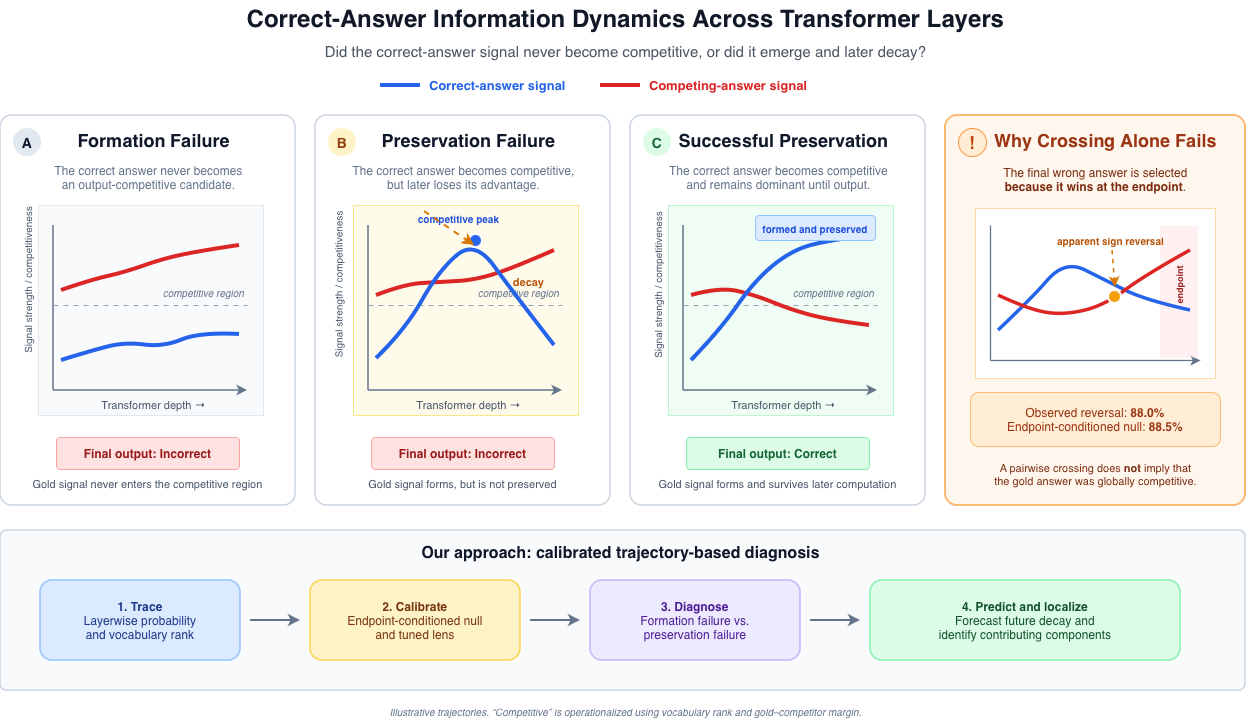
\includegraphics[width=0.9\textwidth]{figures/fig1_concept.png}
\caption{Conceptual overview. When an LLM outputs an incorrect answer, internal representations may either fail to form a competitive gold-answer signal (\emph{formation failure}) or build a competitive signal at intermediate layers that decays before the final layer (\emph{preservation failure}). Our calibrated framework traces these dynamics across layers.}
\label{fig:concept}
\end{figure}

Recognizing these two cases is harder than it looks (Figure~\ref{fig:concept}). Operationally, we call the correct-answer signal \emph{competitive} at a layer if the gold answer enters the top region of the vocabulary distribution and holds a positive margin over competing tokens; a formation failure never achieves this at any intermediate layer, while a preservation failure achieves it and then loses the advantage by the output layer. A common shortcut decodes intermediate hidden states (e.g., via logit lens \citep{nostalgebraist2020logitlens}) and checks whether the gold answer ever outranks the final wrong answer. We show this shortcut is fundamentally misleading for two reasons. First, pairwise crossing is trivially weak: a random-competitor null produces an even higher crossing rate (98.8\% vs.\ 92.2\% observed), so almost any token is temporarily outranked by gold regardless of whether the gold signal was ever competitive. Second, applying the final output head to intermediate states misreads the signal, because early hidden states occupy a different vector space than the output layer \citep{belrose2023tunedlens, din2023jump}.

To reliably diagnose model errors, we introduce \emph{Information Dynamics}, a framework that tracks how the correct answer evolves layer by layer: for each input we measure, at every layer, the gold answer's log-probability, full-vocabulary rank, and margin over competing candidates, paired with a randomized null baseline (to rule out chance flips) and a tuned lens \citep{belrose2023tunedlens} (to decode intermediate states fairly). Across six LLMs (4B--14B) and seven tasks, the framework shows that most errors are formation failures, that preservation failures are a small, task-dependent subset concentrated in short-answer factual tasks, that early-trajectory prefixes predict subsequent decay, and that the taxonomy is causally grounded: preservation failures are differentially repairable by restoring the signal that late-layer computation removed.

Our contributions are:
\begin{enumerate}
    \item \textbf{Shortcut invalidation:} uncorrected pairwise sign flips cannot establish prior signal competitiveness; strength-matched nulls produce even higher crossing rates.
    \item \textbf{Calibrated failure taxonomy:} a strict rank-plus-margin criterion (validated with a teacher-forced sequence-level protocol) under which preservation failures are a task-dependent minority.
    \item \textbf{Predictive trajectory dynamics:} early trajectory history forecasts later decay (AUC 0.75 linear / 0.92 nonlinear) beyond snapshot and final-layer confidence baselines, with cross-task and cross-model transfer.
    \item \textbf{Causal validation and differential repairability:} a four-step causal chain -- peak-state restoration, rank-matched restoration, gold-direction patching, and component-selective patching with orthogonal nulls -- shows the decayed gold signal can be causally restored, and selective intervention guided by a leak-audited non-oracle predictor improves per-intervention efficiency by 67\% at 20\% budget.
    \item \textbf{Benchmark:} we release \texttt{InfoDyn-Bench}, layered information trajectories, derived metrics, and failure labels across six models and seven tasks.
\end{enumerate}

\section{Related Work}
\label{sec:related}

\paragraph{Decoding and probing intermediate representations.}
Logit lens \citep{nostalgebraist2020logitlens}, tuned lens \citep{belrose2023tunedlens}, probing classifiers \citep{alain2016understanding, tenney2019bert, hewitt2019structural, belinkov2022probing}, and early-exit work \citep{schuster2022confident, din2023jump} ask whether a signal is \emph{present} at a layer; we study how the correct-answer signal \emph{evolves dynamically} and quantify readout and selection biases. Knowledge-localization and model-editing work \citep{geva2021transformer, dai2022knowledge, meng2022rome, meng2023memit} locates static facts; we track the rise and decay of the answer signal along depth.

\paragraph{Hallucination and error prediction.}
Uncertainty estimation and hidden-state failure prediction analyze intermediate representations for errors \citep{kadavath2022language, burns2022discovering, azaria2023internal, yin2023do, manakul2023selfcheckgpt}. Closest to us, \citet{jiang2024hallucination} and \citet{kim2025uncertainty} study layer-wise dynamics of correct versus hallucinated outputs. We differ in that (i) we show naive pairwise crossings are explained by selection bias and add the calibration step prior analyses lack; (ii) we split errors into an operational formation-versus-preservation taxonomy; and (iii) we test predictive power against temporal-extrapolation baselines.

\paragraph{Mechanistic interpretability and intervention.}
Circuit analysis, direct logit attribution, and activation patching decompose computations into components \citep{elhage2021mathematical, olsson2022incontext, wang2022interpretability, nanda2023progress}; representation engineering modifies hidden states to steer behavior \citep{turner2023activation, rimsky2023steering, zou2023representation}. We use these tools to causally validate a failure taxonomy rather than to propose a steering method.

\section{Problem Definition}
\label{sec:def}

\subsection{Setup}
Let $x$ be a question, $y^\star$ the gold-answer token, and $\hat{y}$ the generated token. At layer $\ell$ ($1 \le \ell \le L$), let $h_\ell(x) \in \mathbb{R}^d$ be the hidden state at the target position, and let $w_y$ be the unembedding vector of token $y$. A lens $g_\ell$ maps the representation to logits, softmaxed into $p_\ell(y \mid x)$. The raw logit lens sets $g_\ell$ to the final language-model head; the tuned lens \citep{belrose2023tunedlens} adds a per-layer affine map trained to approximate the final-layer logits (Appendix~\ref{app:impl}). The \emph{gold rank} $r_\ell(y^\star)$ is the number of tokens whose probability exceeds the gold answer's (zero-based; $r=0$ means top-1).

\subsection{Margins and Trajectory}
We use two margins: against the generated answer, $\mathrm{CIS}^{\mathrm{gen}}_\ell = \log p_\ell(y^\star) - \log p_\ell(\hat{y})$ (endpoint-bias analysis), and against the strongest final-layer competitor $y^- = \arg\max_{y \neq y^\star} p_L(y)$,
\begin{equation}
\mathrm{CIS}^{\mathrm{comp}}_\ell = \log p_\ell(y^\star) - \log p_\ell(y^-).
\label{eq:cis}
\end{equation}
We fix $y^-$ across all layers so the margin tracks a consistent comparison; a per-layer competitor would collapse the margin test to ``gold is rank-1,'' which is too strict. The \emph{information trajectory} is the per-layer collection $\mathcal{T}(x) = \{\log p_\ell(y^\star), r_\ell(y^\star), \mathrm{CIS}^{\mathrm{comp}}_\ell\}_{\ell=1}^{L}$, from which we derive the \emph{peak rank} $r_{\mathrm{peak}} = \min_{\ell < L} r_\ell(y^\star)$ and the \emph{peak-to-final decay} $D = \max_{\ell < L} \mathrm{CIS}^{\mathrm{comp}}_\ell - \mathrm{CIS}^{\mathrm{comp}}_L$. Appendix~\ref{app:metric} states which margin each analysis uses.

\subsection{Error Taxonomy}
The \emph{competitive decay} label marks an error whose gold answer is competitive at some intermediate layer but negative at the final layer:
\begin{equation}
C(x) = \mathbb{1}\Big[ \exists\, \ell < L : r_\ell(y^\star) \le k \;\land\; \mathrm{CIS}^{\mathrm{comp}}_\ell > 0 \Big] \cdot \mathbb{1}\Big[ \mathrm{CIS}^{\mathrm{comp}}_L < 0 \Big] .
\label{eq:tax}
\end{equation}
We use $k=5$: entering the top-$k$ marks a robust transition in decodability -- the gold log-probability jumps by about $+8$ logits (from noise level $\approx -11$ to $\approx -2.7$) at that moment, in 97\% of samples (Appendix~\ref{app:thresholds}). Under this criterion a \emph{formation failure} never satisfies Eq.~\ref{eq:tax}'s first indicator at any intermediate layer; a \emph{preservation failure} satisfies it and loses the advantage by the final layer; correct examples with a maintained signal are \emph{successful preservations}; the rest are \emph{unresolved} (e.g., multi-step reasoning where the final-answer token alone cannot describe the error).

\paragraph{Multi-token answers.}
For multi-token answers we define the answer-level rank $r^{\mathrm{multi}}_\ell = \min_i r_\ell(y^\star_i)$ (permissive), and, as our main sequence-level criterion, a teacher-forced protocol that appends the gold answer to the prompt and requires aggregation rules applied consistently at every layer: \textbf{ALL} (every answer token top-$k$ at the same intermediate layer), \textbf{MEAN}, and \textbf{JOINT} (protocol details in Appendix~\ref{app:teacherforced}). The minimum-over-tokens rule is a permissive upper bound only: across all 1{,}494 Qwen3-8B errors it yields 90.6\% versus 13.2\% under ALL, and the ALL rate decreases monotonically with answer length (24.3\% / 13.5\% / 11.9\% for one / two / three-plus tokens) -- exactly the length bias the permissive rule introduces. All headline analyses use the first-token or ALL-based criteria.

\section{Experimental Setup}
\label{sec:setup}

We evaluate six open-weight instruction-tuned models -- Qwen3-14B/8B/4B, Qwen2.5-7B, Llama-3.1-8B \citep{dubey2024llama}, and Mistral-7B-Instruct-v0.3 \citep{jiang2023mistral} -- on seven tasks: TriviaQA \citep{joshi2017triviaqa}, HotpotQA \citep{yang2018hotpotqa}, GSM8K \citep{cobbe2021gsm8k}, CommonsenseQA, ARC-Challenge, QuALITY, and MMLU (four subjects). Correctness is exact substring match after normalization (numeric comparison for math; any alias counts for TriviaQA). Tuned-lens translators are trained per layer on unlabelled prompts to predict the model's own final-layer logits, so no answer or correctness labels reach the lens (details in Appendix~\ref{app:impl}). We report bootstrap 95\% confidence intervals for key proportions and per-task/per-model numbers alongside aggregates.

\section{Results: Measurement}
\label{sec:results}

\subsection{Pairwise Sign Flips Fail to Establish Signal Competitiveness}
\label{sec:null}

Across error examples, the gold token's log-probability surpasses the final competitor at some intermediate layer in 92.2\% of cases. To assess whether this is meaningful we construct two nulls: a \emph{random-competitor null} (replace the true competitor with a token generated for a different, randomly selected error) and a \emph{rank-matched null} (replacement competitors within $\pm 1$ logit of the true competitor's final-layer strength). Under both nulls the crossing rate is even higher -- 98.8\% $\pm$ 0.4\% and 98.7\% $\pm$ 0.4\% (200 permutations, 95\% CI [98.0\%, 99.6\%]) -- so almost any token is crossed by gold at some layer regardless of competitor strength (Figure~\ref{fig:bias}a). Pairwise crossings therefore offer no evidence that a gold signal ever formed. In addition, projecting intermediate states through the final head inflates peak intermediate margins by ${\sim}2\times$ relative to a calibrated readout (median peak margin 4.53 vs.\ 2.24; Figure~\ref{fig:bias}b), reinforcing that uncalibrated pairwise leads are uninterpretable.

\begin{figure}[t]
\centering

\includegraphics[width=0.95\textwidth]{figures/fig2_measurement_bias.pdf}
\caption{Measurement bias. Left: the observed pairwise crossing rate (92.2\%) is lower than both nulls (98.8\%, 98.7\%), showing crossing is trivially weak. Right: the raw logit lens inflates intermediate peak margins by ${\sim}2\times$ relative to the tuned lens. All left-panel numbers are read directly from the matched-null analysis output.}
\label{fig:bias}
\end{figure}

\subsection{Correct and Incorrect Outputs Follow Distinct Trajectories}
\label{sec:traj}

Correct predictions establish a strong, persistent gold signal early; incorrect predictions show weak formation and substantial late-layer decay (Figure~\ref{fig:trajectories}). Median intermediate peak ranks for correct outputs reach top positions across models (e.g., 0 for Qwen3-8B, 1 for Llama-3.1-8B, 11 for Mistral-7B), versus 19, 20, and 77 for incorrect outputs; 90.5\% of correct Qwen3-8B examples enter the top-5 at some intermediate layer versus 26.4\% of incorrect ones (Table~\ref{tab:rank}). The separation is not an artifact of any single decoder: raw lens, tuned lens, and a parameter-free cosine-similarity decoder all separate correct from incorrect by over an order of magnitude in rank ($p < 10^{-20}$; Appendix~\ref{app:probe}).

\begin{table}[t]
\centering
\caption{Median peak rank (excluding the final layer) and top-5 entry rate for correct versus incorrect predictions.}
\label{tab:rank}
\small
\begin{tabular}{lcccc}
\toprule
\textbf{Model} & \multicolumn{2}{c}{\textbf{Correct}} & \multicolumn{2}{c}{\textbf{Incorrect}} \\
\cmidrule(lr){2-3}\cmidrule(lr){4-5}
 & Peak Rank & Top-5 Entry & Peak Rank & Top-5 Entry \\
\midrule
Qwen3-14B & 1 & \cdot & 9 & \cdot \\
Qwen3-8B & 0 & 90.5\% & 19 & 26.4\% \\
Qwen3-4B & 2 & \cdot & 10 & \cdot \\
Qwen2.5-7B & 1 & \cdot & 26 & \cdot \\
Llama-3.1-8B & 1 & 79.6\% & 20 & 26.7\% \\
Mistral-7B & 11 & 30.2\% & 77 & 8.4\% \\
\bottomrule
\end{tabular}
\end{table}

\begin{figure}[t]
\centering
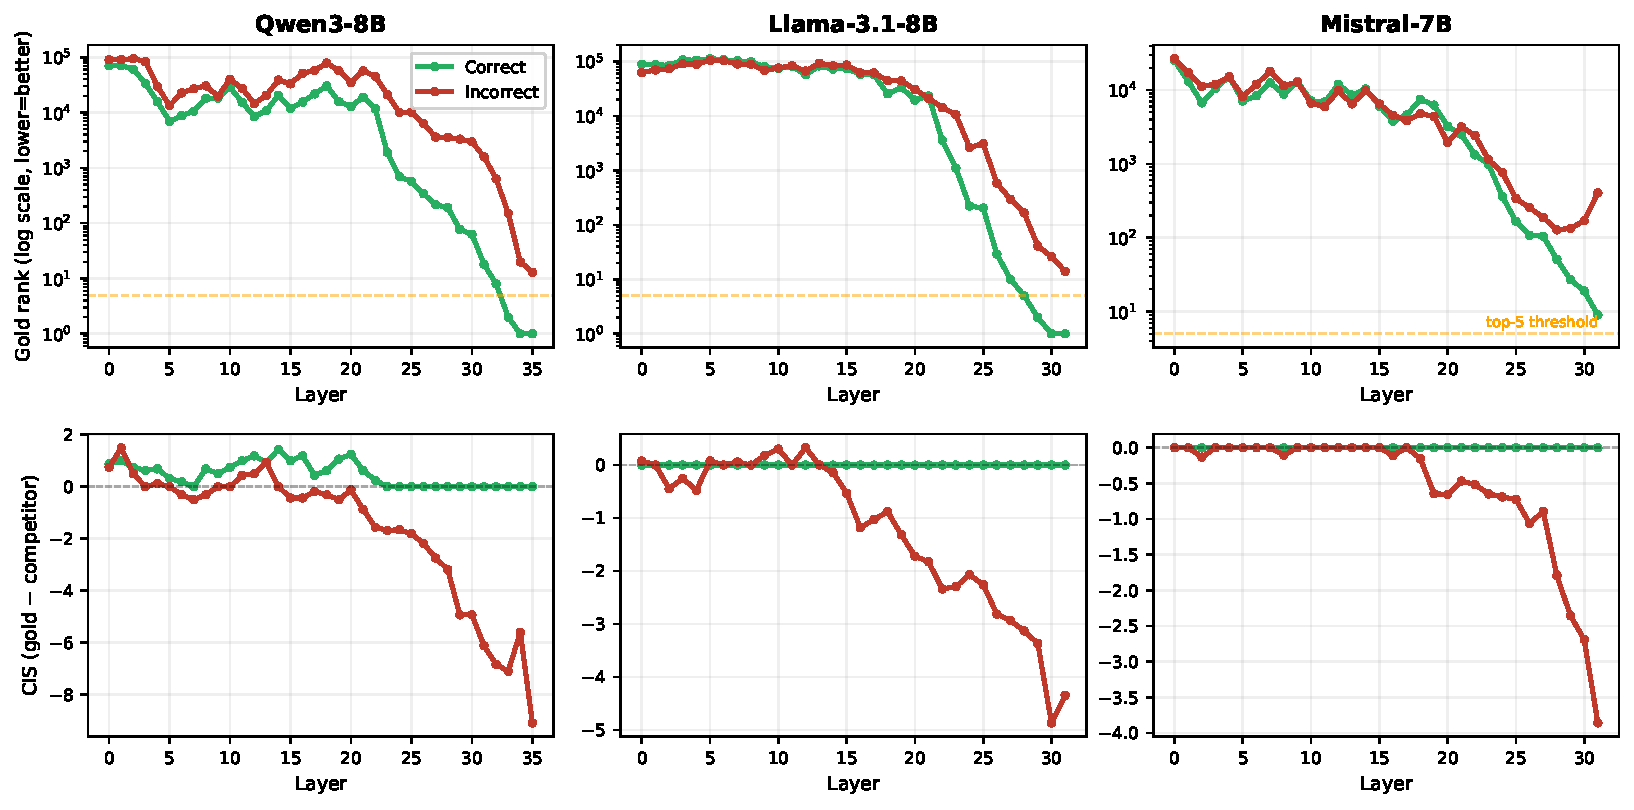
\includegraphics[width=0.95\textwidth]{figures/fig3_trajectories.pdf}
\caption{Median gold-answer rank (top, log scale) and probability margin (bottom) across layers for correct (green) and incorrect (red) predictions.}
\label{fig:trajectories}
\end{figure}

\subsection{Preservation Failures Are a Small, Task-Dependent Minority}
\label{sec:minority}

Applying the strict criterion (Eq.~\ref{eq:tax}) to all 1{,}494 Qwen3-8B errors yields an overall preservation-failure rate of 10.0\% (95\% CI [8.4\%, 11.4\%]), consistent with the tuned-lens calibrated subset (8.9\%, CI [6.4\%, 11.5\%]) and clearly task-structured: multi-hop QA 14.2\% [9.5, 19.5], world knowledge 12.6\% [7.8, 18.0], long-context comprehension 12.1\% [8.0, 16.6], knowledge QA 12.0\% [8.5, 15.9], science reasoning 10.9\% [7.0, 14.8], commonsense 9.2\% [5.6, 13.3], math 0.0\%. Table~\ref{tab:taskdecay} reports the main answer-level metric -- the strict teacher-forced ALL-based sequence-level rate -- alongside the permissive minimum-over-tokens rate as an upper bound. Under the strict sequence-level criterion, multi-hop QA (24.2\%) and knowledge QA (23.0\%) are highest, math (4.3\%) and long-context comprehension (0.5\%) lowest. The two metrics diverge most on long answers: long-context comprehension ranks second-highest under the permissive rule (27.6\%) yet drops to 0.5\% under ALL, because with many answer tokens the ``any token ever top-5'' criterion is trivially easy -- the formation that occurs is fragmentary, covering individual tokens rather than the full sequence. The two strict criteria diverge informatively in the same direction (Eq.~\ref{eq:tax} scores the first answer token: 12.1\% on long-context; ALL requires every token: 0.5\%): first tokens form on long answers, full sequences do not. Preservation failures with sequence-level integrity are therefore concentrated in short-answer factual tasks; procedural computation either succeeds or never forms the final-answer signal (GSM8K's low rate is unchanged under multi-token tracking; Appendix~\ref{app:thresholds}). The taxonomy is stable under the competitiveness threshold ($k{=}1 \to 50$: 4.8\% $\to$ 16.9\%; Appendix~\ref{app:thresholds}) and under the choice of lens (Appendix~\ref{app:probe}), and the lens carries no label leakage (Appendix~\ref{app:probe}).

\begin{table}[t]
\centering
\caption{Preservation rate by task on Qwen3-8B (1{,}494 errors). Main metric: strict teacher-forced sequence-level criterion (ALL -- every gold-answer token simultaneously top-5 at some intermediate layer; overall 13.2\%). Upper bound: permissive min-over-tokens rule (any gold token ever entering top-5 then falling below rank 10; overall 90.6\%), which inflates rates with answer length.}
\label{tab:taskdecay}
\small
\begin{tabular}{lcccc}
\toprule
\textbf{Task} & \textbf{Type} & \textbf{Errors} & \textbf{ALL (main)} & \textbf{Min-rule (bound)} \\
\midrule
HotpotQA & Multi-hop QA & 190 & 24.2\% & 26.3\% \\
TriviaQA & Knowledge QA & 283 & 23.0\% & 27.9\% \\
MMLU & World knowledge & 167 & 16.8\% & 23.4\% \\
ARC-Challenge & Science reasoning & 229 & 12.2\% & 23.6\% \\
CommonsenseQA & Commonsense & 196 & 9.7\% & 12.2\% \\
GSM8K & Math reasoning & 230 & 4.3\% & 5.2\% \\
QuALITY & Long-context & 199 & 0.5\% & 27.6\% \\
\midrule
\textbf{Overall} & --- & 1{,}494 & \textbf{13.2\%} & 90.6\% \\
\bottomrule
\end{tabular}
\end{table}

\section{Results: Prediction}
\label{sec:prediction}

If the measured dynamics capture how a model forms and maintains answers, the trajectory prefix should predict future decay. We train a classifier on features from the first half of the network only, predicting the second-half decay label $y^{\mathrm{decay}} = \mathbb{1}[\max_{\ell \ge t_0} \mathrm{CIS}^{\mathrm{comp}}_\ell > 0 \,\land\, \mathrm{CIS}^{\mathrm{comp}}_L < 0]$; the label uses only second-half information, strictly separating it from the features. On Qwen3-8B, L2-regularized logistic regression reaches AUC 0.75 $\pm$ 0.02 (5-fold CV, 95\% CI [0.70, 0.80]; single split 0.79; PR-AUC 0.71 at a 46\% positive rate), versus 0.39--0.61 for midpoint snapshot baselines (margin, rank, entropy) and simple summaries (margin-plus-slope, running max). A random forest reaches 0.92 $\pm$ 0.01 (permutation $p < 0.02$); we report the linear number as a conservative bound. The trajectory prefix also exceeds \emph{final-layer} confidence baselines (combined margin/rank/entropy: 0.70 vs.\ 0.78), although the baselines observe the fully executed computation -- early history contains dynamic signal the output confidence lacks (Figure~\ref{fig:prediction}a). The gain is not temporal autocorrelation: persistence, slope, and autoregressive forecasts from the first half reach only 0.56--0.62 (Appendix~\ref{app:prediction}), and an endpoint-free variant using only gold-token features still reaches 0.66. Prediction transfers in a structure-dependent way across tasks (entity QA $\to$ multi-hop QA 0.74; multi-hop $\to$ math 0.77; single-step recall $\to$ math 0.38) and across model families (leave-one-model-out mean 0.739; Appendix~\ref{app:prediction}).

\begin{figure}[t]
\centering

\includegraphics[width=0.95\textwidth]{figures/fig5_prediction.pdf}
\caption{Decay prediction. (a) Within-task AUC: full trajectory vs.\ snapshot and final-layer baselines. (b) Cross-task transfer. (c) Cross-model transfer.}
\label{fig:prediction}
\end{figure}

\paragraph{An inference-available predictor.}
\label{sec:nonoracle}
The trajectory features above reference the gold token, which is unavailable at deployment. We therefore trained a predictor using \emph{only} the model's own top-5 distributions over the first half of layers, with every feature audited to be strictly prefix-only (leader churn, prefix-leader hold anchored at the mid-network top-1, top-1/top-2 margin dynamics, top-5 entropy and mass). A random forest predicts preservation failures with pooled out-of-fold ROC-AUC 0.669 (bootstrap 95\% CI [0.630, 0.709]; PR-AUC 0.383 vs.\ a 0.294 base rate), with leader churn most informative; flagging the top 20\% of errors yields 1.35$\times$ precision lift. In deployment the trigger is calibrated once on labeled errors covering the target task distribution -- the setting the pooled out-of-fold AUC measures -- after which it needs no gold information. We use this trigger to drive a real intervention in Section~\ref{sec:causal}.

\section{Results: Causal Validation and Intervention}
\label{sec:causal}

We first locate the suppression, then validate it causally at four levels of specificity, summarized in Table~\ref{tab:causal}.

\paragraph{Attribution: the suppression lives in the late-layer MLPs.}
Direct logit attribution assigns each layer's MLP output $m_\ell$ the margin contribution $(w_{y^\star} - w_{y^-})^\top m_\ell$; decomposing the per-layer margin change into attention and MLP parts, the MLP dominates for incorrect examples (cumulative $-4.71$ vs.\ $-3.42$), with the layer-35 MLP the largest single negative source ($-3.42$), agreed on by both methods (Figure~\ref{fig:intervention}b), while correct examples show no dominant negative component ($-0.52$/$-0.51$). Removing the gold direction from late-layer hidden states also flips 40--87\% of correct examples to wrong across all six models, versus ${\approx}0\%$ for norm-matched controls (Figure~\ref{fig:intervention}a; Appendix~\ref{app:ablation}) -- the gold direction is behaviorally necessary.

\begin{figure}[t]
\centering
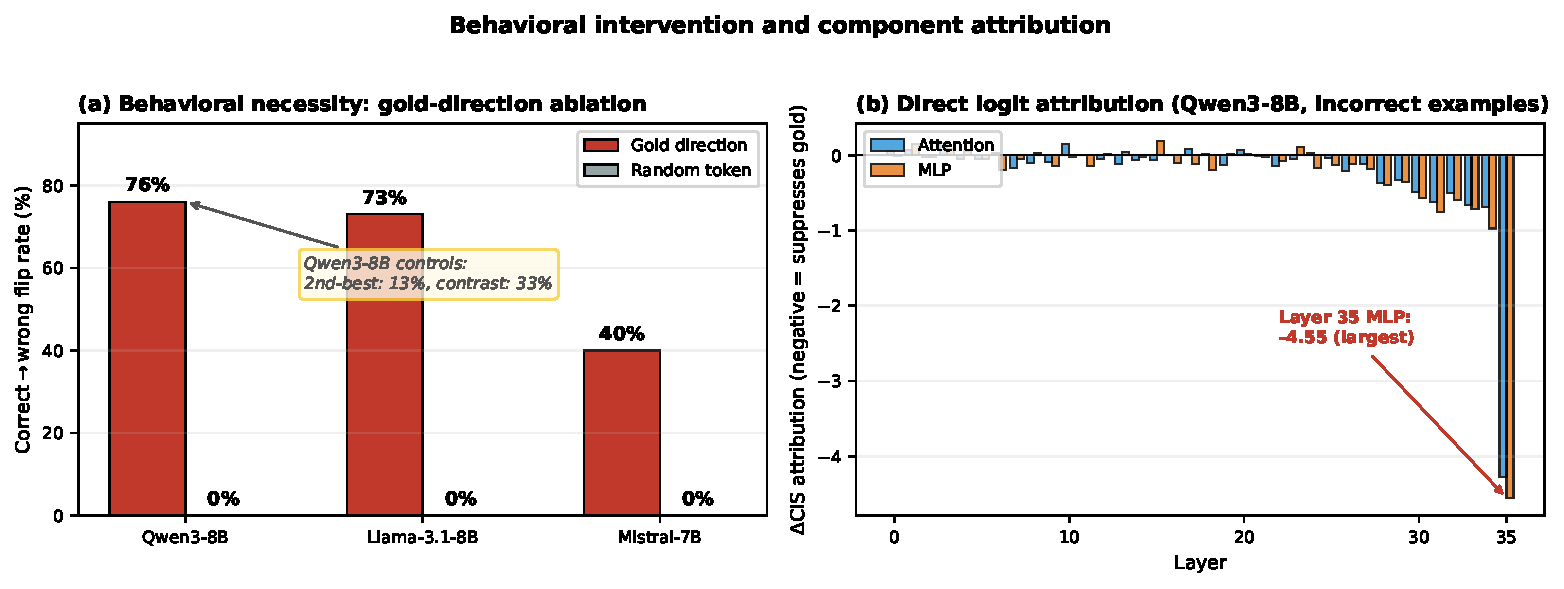
\includegraphics[width=0.95\textwidth]{figures/fig6_intervention.pdf}
\caption{(a) Ablating the gold direction flips correct examples to wrong across model families and scales while controls flip almost none. (b) Per-layer attention/MLP contribution to the margin (Qwen3-8B, incorrect examples): the late-layer MLP carries the largest negative attribution.}
\label{fig:intervention}
\end{figure}

\paragraph{Peak-state restoration: the intermediate signal is causal.}
For each error we find the layer $L^\star$ where the gold rank peaked, capture the last-token residual there, and for every later layer blend the residual toward the peak state, $h'_\ell = (1-\alpha) h_\ell + \alpha h_{L^\star}$ -- an intervention blind to the final-layer distribution. At $\alpha = 0.8$, preservation failures recover at 8.3\% versus 3.3\% for formation (2.5$\times$); at $\alpha=0.5$ the effect is preservation-exclusive (5.0\% vs.\ 0.0\%).

\paragraph{Rank-matched restoration: not a final-rank artifact.}
Matching each preservation failure to a true formation failure (peak rank $> 20$) with the same final rank ($\pm 3$) equalizes the output distance (final-rank medians 8 vs.\ 11) while preserving the peak contrast (3 vs.\ 31). At $\alpha = 1$ the restoration recovers 12.3\% of preservation versus 1.8\% of formation failures (7.0$\times$, 57 pairs), strengthening monotonically with $\alpha$ ($3.0\times/6.0\times/7.0\times$) while the formation rate stays flat. Because the design is paired we do not claim significance at this sample size: paired bootstrap CI $[1.8\%, 19.3\%]$, exact McNemar $p = 0.070$ (7 vs.\ 1 discordant pairs); the decisive statistical test comes next.

\paragraph{Gold-direction patching: significant, direction-specific.}
Patching at every layer after $L^\star$ the gold-direction component that decayed from the peak state, $h'_\ell = h_\ell + \beta\,\mathrm{clamp}_{\ge 0}((h_{L^\star} - h_\ell)^\top \hat{w}_{y^\star})\,\hat{w}_{y^\star}$, we measure the \emph{net} recovery rate (not top-1 at baseline $\to$ top-1 after patch). On $n{=}300$ ($\beta{=}4$), the gold patch recovers 7.3\% of preservation failures versus 0.7\% of formation failures (10.9$\times$; Fisher $p = 0.005$) and 0.0\% of a matched-null control restoring a random competitor direction \emph{orthogonalized against gold} (0/109; $p = 0.003$). The decayed gold-direction signal is causal: restoring it reinstates the answer for preservation failures and does nothing for formation failures that never carried it.

\paragraph{Component-selective patching: distributed suppression.}
Finally we patch a \emph{single component at a single layer}, deleting the margin-suppressive part of the write, $m' = m - \gamma\,\mathrm{clamp}_{\le 0}(m^\top \hat{d})\,\hat{d}$, with $\hat{d}$ the unit gold-vs-competitor contrast direction. Removing this component from the layer-35 MLP alone recovers 11.0\%/20.2\%/31.2\% of preservation failures at $\gamma = 1/2/4$, while a random orthogonal direction recovers exactly 0/109 at every strength ($p < 0.001$): the effect is specific to the margin direction. The same patch on adjacent MLPs recovers similarly (layer 34: 12.8--33.0\%; layer 33: 11.9--25.7\%), with no significant difference between layers 35 and 34 ($p \ge 0.67$), and full zero-ablation of the layer-35 MLP \emph{worsens} the mean gold rank ($-13.0$) because the component also carries essential non-suppressive computation. The suppression is thus causal and direction-selective but \emph{distributed} across the final MLPs (31--35); the DLA ranking reflects direct-effect magnitude, not unique causal necessity.

\begin{table}[t]
\centering
\caption{Causal validation summary (Qwen3-8B preservation failures; net recovery unless noted). Each step adds a control dimension: intermediate vs.\ output locus, final-rank confound, direction specificity, and component specificity.}
\label{tab:causal}
\small
\begin{tabular}{llcc}
\toprule
\textbf{Experiment} & \textbf{Control} & \textbf{Preserv.} & \textbf{Formation / null} \\
\midrule
Peak restoration ($\alpha{=}0.8$) & balanced groups & 8.3\% & 3.3\% (2.5$\times$) \\
Rank-matched ($\alpha{=}1$) & final rank matched & 12.3\% & 1.8\% (7.0$\times$, $p{=}.070$) \\
Gold-direction patch ($\beta{=}4$) & orthogonal null & 7.3\% & 0.7\% / 0.0\% ($p{=}.005$) \\
Component patch ($\gamma{=}4$) & rand.\ orth.\ / neighbors & 31.2\% & 0.0\% ($p{<}.001$) \\
\bottomrule
\end{tabular}
\end{table}

\paragraph{Differential repairability under steering, and a closed loop.}
The taxonomy also identifies \emph{differentially repairable} errors. Under a calibrated logit bonus (oracle proof-of-concept; Appendix~\ref{app:steering}), preservation failures recover at 4--5$\times$ the formation rate. Under a Representation-Engineering steering pipeline whose trigger is the trajectory predictor, selective steering achieves 9.1\% recovery per intervention versus 4.0\% indiscriminate (127\% efficiency gain, 72\% budget saved), with the ground-truth differential at 3.7$\times$ (6.6\% vs.\ 1.8\%). Replacing the oracle-assisted trigger with the strictly non-oracle predictor of Section~\ref{sec:nonoracle} -- calibrated per task, out-of-fold, evaluated on a task-balanced set (30 errors/task) -- selective steering at 20\% coverage recovers 9.5\% per intervention versus 5.7\% indiscriminate (67\% gain, 80\% budget saved), flags preservation failures at 64\% precision against a 33\% base rate (1.9$\times$ lift), and preserves the differential signature (8.6\% vs.\ 4.3\%, 2.0$\times$). The closed loop runs without any gold-conditioned feature at test time and retains about half the oracle-assisted efficiency gain.

\section{InfoDyn-Bench}
\label{sec:bench}

We release \texttt{InfoDyn-Bench}: for each example, the full per-layer gold trajectory under raw and tuned lenses, derived dynamics metrics (signal-emergence layer, peak rank/CIS, dwell time, decay), failure-pattern labels, and a decay-prediction split, across six models $\times$ seven tasks (contents in Appendix~\ref{app:bench}). The benchmark directly supports error-mechanism studies, decay-prediction research without re-running models, and intervention/probing evaluation; we include a dataset card, licenses, and reproduction scripts.

\section{Discussion and Limitations}
\label{sec:discussion}

Competitive decodability is an operational sign of output readiness, not a complete definition of knowledge; we do not equate a top-5 rank with ``knowing.'' The failure types call for different responses -- formation failures may need retrieval or knowledge editing \citep{meng2022rome}, preservation failures suit retention-style intervention \citep{turner2023activation, zou2023representation} -- and Section~\ref{sec:causal} provides causal, component-selective evidence for such interventions, though scaling them into a practical repair method remains future work. We conjecture trajectories predict because slope reflects stability, early peaks reflect formation speed, and fluctuation reflects competitiveness -- history separates transient fluctuation from stable formation better than any snapshot. Limitations: the margin is a proxy, not knowledge itself; final-answer-token tracking does not fully describe multi-step reasoning; multi-token answers are harder to measure (our ALL criterion is conservative); the tuned lens may carry probe bias; the taxonomy depends on a threshold, though slowly; and our scale analysis covers 4B--14B across three families, so we do not claim generality beyond this range.

\section{Conclusion}

We showed that the same final error can arise from different internal dynamics: a correct-answer signal that never forms, or one that forms and then decays. Naive pairwise crossings overstate the second case because of endpoint selection and readout biases. After calibration, a small, task-dependent preservation-failure regime emerges, concentrated in short-answer factual tasks; it is predictable from early trajectories, causally repairable, and targetable by a leak-audited non-oracle trigger. We release \texttt{InfoDyn-Bench} to support further study of process-level error diagnosis.

\bibliography{iclr2027_conference}
\bibliographystyle{iclr2027_conference}

\appendix

\section{Metric Usage}
\label{app:metric}
Table~\ref{tab:metric} states which margin each analysis uses, so the measurement object is never ambiguous.

\begin{table}[h]
\centering
\caption{Which margin each analysis uses.}
\label{tab:metric}
\begin{tabular}{ll}
\toprule
\textbf{Analysis} & \textbf{Margin} \\
\midrule
Endpoint selection bias & $\mathrm{CIS}^{\mathrm{gen}}$ \\
Correct versus incorrect comparison & $\mathrm{CIS}^{\mathrm{comp}}$ \\
Competitive-decay classification & $\mathrm{CIS}^{\mathrm{comp}}$ \\
Trajectory prediction & $\mathrm{CIS}^{\mathrm{comp}}$ \\
Direct logit attribution & $\mathrm{CIS}^{\mathrm{comp}}$ \\
\bottomrule
\end{tabular}
\end{table}

\section{Teacher-Forced Multi-Token Protocol}
\label{app:teacherforced}
We append the gold answer to the prompt (teacher forcing) and, for each answer token, read the hidden state at the position that predicts it, decoding the gold rank and log-probability at every layer. We aggregate across answer positions with rules applied consistently at every layer: \textbf{ALL} (every answer token top-$k$ at the same intermediate layer), \textbf{MEAN} (mean per-token rank top-$k$), \textbf{JOINT} (intermediate sequence log-likelihood exceeds the final one), and the permissive \textbf{MIN} (any token ever top-$k$; upper bound only). On all 1{,}494 Qwen3-8B errors: ALL 13.2\%, MEAN 25.0\%, JOINT 87.8\%, MIN 90.6\%. The ALL rate decreases monotonically with answer length (24.3\% single-token, 13.5\% two-token, 11.9\% three-plus), confirming the length bias of the minimum rule; the divergence is starkest on long-context comprehension (ALL 0.5\% vs.\ MIN 27.6\%).

\section{Probe Robustness and Label Leakage}
\label{app:probe}
\paragraph{Three independent decoders.}
We recomputed peak intermediate ranks under the raw logit lens, the tuned lens, and a parameter-free cosine similarity between intermediate hidden states and unembedding vectors. Correct and incorrect predictions remain separated by over an order of magnitude in rank under all three decoders (medians 0 vs.\ 32 raw, 0 vs.\ 12 tuned, 1 vs.\ 43 cosine; Mann-Whitney $p < 10^{-20}$ in all cases). Because cosine similarity uses no learned parameters or final layer normalization, the separation is not an artifact of any single decoder.

\paragraph{Zero label leakage.}
The tuned-lens translators are trained strictly on unlabelled general prompts by predicting the model's own final-layer logits, without observing ground-truth answers or correctness labels, so no downstream task information leaks into intermediate readouts. The preservation-failure rate is therefore not a probe artifact.

\paragraph{Raw versus tuned lens agreement.}
The raw lens inflates intermediate peak margins by ${\sim}2\times$, but both lenses yield identical relative orderings between correct and incorrect predictions; calibration adjusts absolute magnitudes without altering the representational dynamics.

\section{Threshold Sensitivity and GSM8K Boundaries}
\label{app:thresholds}
\paragraph{Top-$k$ justification.}
At the first layer where the gold rank drops to $\le k$, the gold log-probability jumps by ${\sim}{+}8$ logits (median $-11 \to -2.7$ at $k{=}5$); the jump is positive in 97\% of samples and large for every $k \in \{1,5,10\}$ (medians $+7.6$, $+8.0$, $+7.5$). Entering the top-$k$ thus marks the transition from vocabulary noise to a decodable candidate.

\paragraph{Sensitivity to $k$.}
Re-evaluating the strict rate across $k \in \{1,5,10,50\}$ on Qwen3-8B with the margin condition fixed gives 4.8\%, 8.5\%, 10.1\%, and 16.9\%: preservation failures remain a small minority at every reasonable threshold.

\paragraph{GSM8K measurement boundaries.}
GSM8K's low rate (5.2\% permissive; 4.3\% strict) is not an artifact of single-token tracking: computing the best rank across all gold-answer tokens reproduces the same rate, since most GSM8K answers are single-token numbers. In multi-step reasoning, incorrect finals stem from intermediate reasoning errors rather than a formed-then-decayed final-answer signal.

\section{Prediction Details}
\label{app:prediction}
\paragraph{Endpoint-free variant.}
Because $\mathrm{CIS}^{\mathrm{comp}}$ references the final-layer competitor, we retrained the predictor using only gold-token features (log-probability, rank, slopes). This endpoint-free predictor reaches AUC 0.66, above all single-layer baselines and temporal-extrapolation baselines, showing the gold trajectory alone carries predictive signal; the full trajectory's 0.75 reflects additional gold-vs-competitor contrast information.

\paragraph{Not temporal autocorrelation.}
Baselines computed from the first half alone: persistence 0.60, linear slope 0.58, extrapolation 0.58, first-order autoregression 0.62, first-half mean 0.56 -- all well below the full trajectory's 0.79. If the signal were autocorrelation, an autoregressive forecast would approach the full model; it does not.

\paragraph{Feature decomposition.}
No single feature matches the full trajectory: margin sign-oscillation count 0.64, first-half peak margin 0.64, first-half variance 0.63, slope 0.61, versus static midpoint margin 0.60 and rank 0.51; peak+slope+variance reach 0.70 and full shape features 0.75 (Figure~\ref{fig:trajdecomp}).

\begin{figure}[h]
\centering
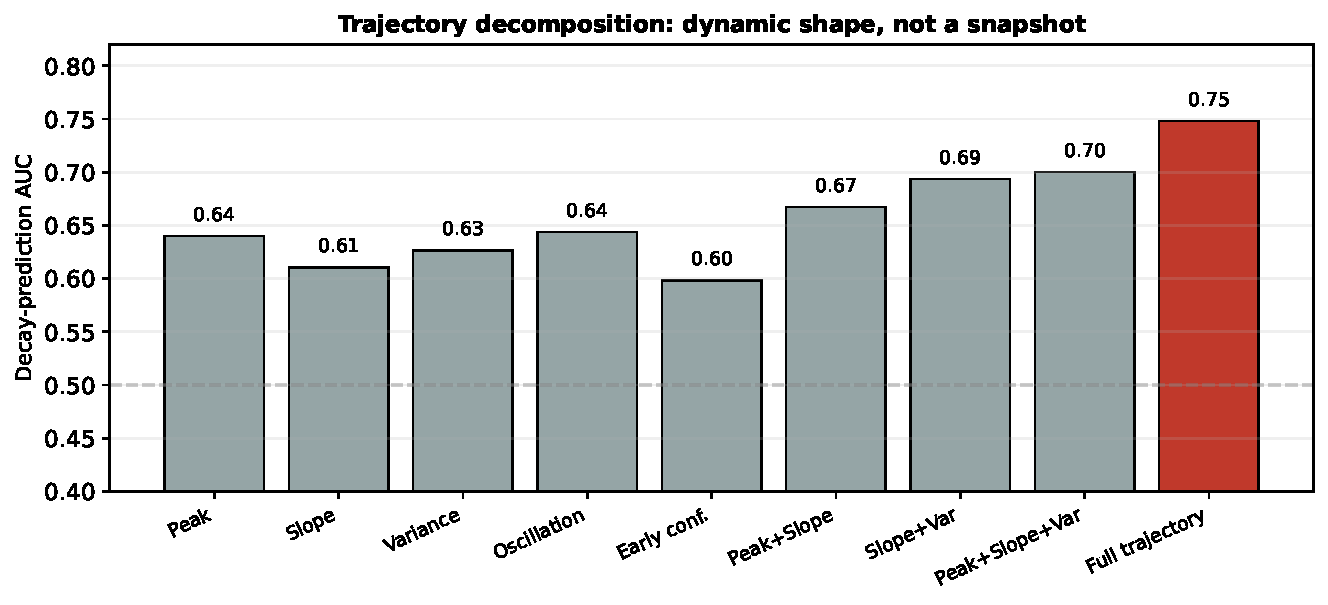
\includegraphics[width=0.8\textwidth]{figures/fig_traj_decomp.pdf}
\caption{Trajectory feature decomposition: dynamic features outperform static snapshots; their combination drives full predictive power.}
\label{fig:trajdecomp}
\end{figure}

\paragraph{Cross-task and cross-model transfer.}
Transfer is structure-dependent: TriviaQA $\to$ HotpotQA 0.74 (0.86 with a random forest), HotpotQA $\to$ GSM8K 0.77, TriviaQA $\to$ GSM8K 0.38, consistent with GSM8K's absent intermediate signals. Cross-model transfer (layers aligned by relative depth, normalization fit on training models only) exceeds chance for all pairs; leave-one-model-out averages 0.739 (Table~\ref{tab:crossmodel}).

\begin{table}[h]
\centering
\caption{Cross-model decay-prediction AUC (rows: training model; columns: test model).}
\label{tab:crossmodel}
\begin{tabular}{lccc}
\toprule
\textbf{Train $\backslash$ Test} & Qwen3-8B & Llama-3.1-8B & Mistral-7B \\
\midrule
Qwen3-8B & \cdot & \textbf{0.728} & 0.748 \\
Llama-3.1-8B & 0.695 & \cdot & 0.779 \\
Mistral-7B & 0.639 & 0.599 & \cdot \\
\midrule
Leave-one-out & 0.703 & 0.750 & 0.763 \\
\bottomrule
\end{tabular}
\end{table}

\section{Gold-Direction Ablation: Necessity and Controls}
\label{app:ablation}
We removed the component of the hidden state along the gold unembedding direction in the last three layers, $h'_\ell = h_\ell - \operatorname{proj}_{w_{y^\star}}(h_\ell)$, applied to originally correct examples. The ablation flips correct examples to wrong at high rates across all models while a random-token control flips almost none (Table~\ref{tab:ablation}): 77\%, 76\%, 67\%, 87\%, 73\%, and 40\% for Qwen3-14B, Qwen3-8B, Qwen3-4B, Qwen2.5-7B, Llama-3.1-8B, and Mistral-7B; the strongest and weakest models' 95\% intervals ([70, 95] vs.\ [25, 58]) do not overlap, so the cross-architecture variation is not sampling noise.

\begin{table}[h]
\centering
\caption{Behavioral necessity: ablating the gold direction flips correct examples to wrong; a random-token control flips almost none. Parentheses: Wilson 95\% intervals.}
\label{tab:ablation}
\small
\begin{tabular}{lccc}
\toprule
\textbf{Model} & \textbf{Baseline correct} & \textbf{Gold flip} & \textbf{Random flip} \\
\midrule
Qwen3-14B & 30/30 & 23/30 (77\%, [59, 88]) & 0/30 (0\%) \\
Qwen3-8B & 50/50 & 38/50 (76\%, [63, 86]) & 0/50 (0\%) \\
Qwen3-4B & 27/27 & 18/27 (67\%, [48, 81]) & 0/27 (0\%) \\
Qwen2.5-7B & 30/30 & 26/30 (87\%, [70, 95]) & 1/30 (3\%) \\
Llama-3.1-8B & 30/30 & 22/30 (73\%, [56, 86]) & 0/30 (0\%) \\
Mistral-7B & 30/30 & 12/30 (40\%, [25, 58]) & 0/30 (0\%) \\
\bottomrule
\end{tabular}
\end{table}

\paragraph{Norm-matched controls.}
Because the gold direction is the main source of the gold log-probability, we matched the perturbation magnitude: each control direction's per-layer removal strength was set so $\lVert \Delta h \rVert$ equals that of the gold ablation. Under this protocol the gold direction still flips far more than any control: on Qwen3-8B, gold 83.3\% vs.\ second-best candidate 38.9\%, random token 5.6\%, random Gaussian direction 11.1\%; on Qwen3-4B, 70.0\%/35.0\%/15.0\%/5.0\%; on Qwen3-14B, 75.0\%/55.0\%/5.0\%/0.0\%. The gradient cannot be explained by a generic large perturbation.

\section{Calibrated Logit-Bonus Steering}
\label{app:steering}
As an oracle proof-of-concept, we added a fixed bonus $\beta$ to the gold token's logit at every decoding step. Preservation failures (gold at final rank $\le 5$ in 91\% of cases, median 1) recover far more than formation failures (median final rank 23): at the ratio-maximizing $\beta = 3$, 30.0\% versus 6.4\% (4.7$\times$); larger bonuses narrow the gap by forcing any token to the top. Sample counts (n${=}40$ preservation, n${=}110$ formation) reflect natural class proportions among the first 150 errors.

\begin{table}[h]
\centering
\caption{Logit-bonus recovery by failure type (oracle proof-of-concept).}
\label{tab:steering}
\begin{tabular}{lccc}
\toprule
\textbf{Bonus $\beta$} & \textbf{Preservation (n=40)} & \textbf{Formation (n=110)} & \textbf{Ratio} \\
\midrule
1.0 & 2.5\% & 0.9\% & 2.8$\times$ \\
2.0 & 12.5\% & 2.7\% & 4.6$\times$ \\
3.0 & 30.0\% & 6.4\% & 4.7$\times$ \\
5.0 & 32.5\% & 11.8\% & 2.8$\times$ \\
\bottomrule
\end{tabular}
\end{table}

\section{InfoDyn-Bench Contents}
\label{app:bench}

\begin{table}[h]
\centering
\caption{Contents of \texttt{InfoDyn-Bench}.}
\label{tab:benchmark}
\small
\begin{tabular}{lp{8.6cm}}
\toprule
\textbf{Component} & \textbf{Description} \\
\midrule
\textbf{Input} & Question, gold answer, aliases, generated answer, correctness label. \\
\textbf{Trajectory} & Per-layer gold-answer log-probability, full-vocabulary rank, margin over the competing token, under both lenses. \\
\textbf{Derived metrics} & Signal-emergence layer, peak rank, peak CIS, dwell time, peak-to-final decay, sign-change flag, top-5 entry. \\
\textbf{Failure label} & \texttt{Absent}, \texttt{Preservation-Failure}, \texttt{Late-Emergent}, \texttt{Decay}, \texttt{Stable}. \\
\textbf{Prediction split} & $t_0$ prefix features, the $y^{\mathrm{decay}}$ label, final correctness. \\
\textbf{Coverage} & 6 models (Qwen3-4B/8B/14B, Qwen2.5-7B, Llama-3.1-8B, Mistral-7B) $\times$ 7 tasks. \\
\bottomrule
\end{tabular}
\end{table}

\section{Implementation Details}
\label{app:impl}
\paragraph{Lens construction.}
For the tuned lens we fit, per layer, an affine map $(\mathbf{A}_\ell, \mathbf{b}_\ell)$ so that $\mathbf{A}_\ell h_\ell + \mathbf{b}_\ell$, decoded through the final norm and head, approximates the final-layer logits; translators are trained independently on a held-out prompt subset (Adam, learning rate $10^{-3}$, 500 epochs), supervised by the model's own final logits rather than answer labels.

\paragraph{Taxonomy figure.}
Figure~\ref{fig:taxonomy} visualizes the operational taxonomy across tasks under the strict criterion (Eq.~\ref{eq:tax}).

\begin{figure}[h]
\centering
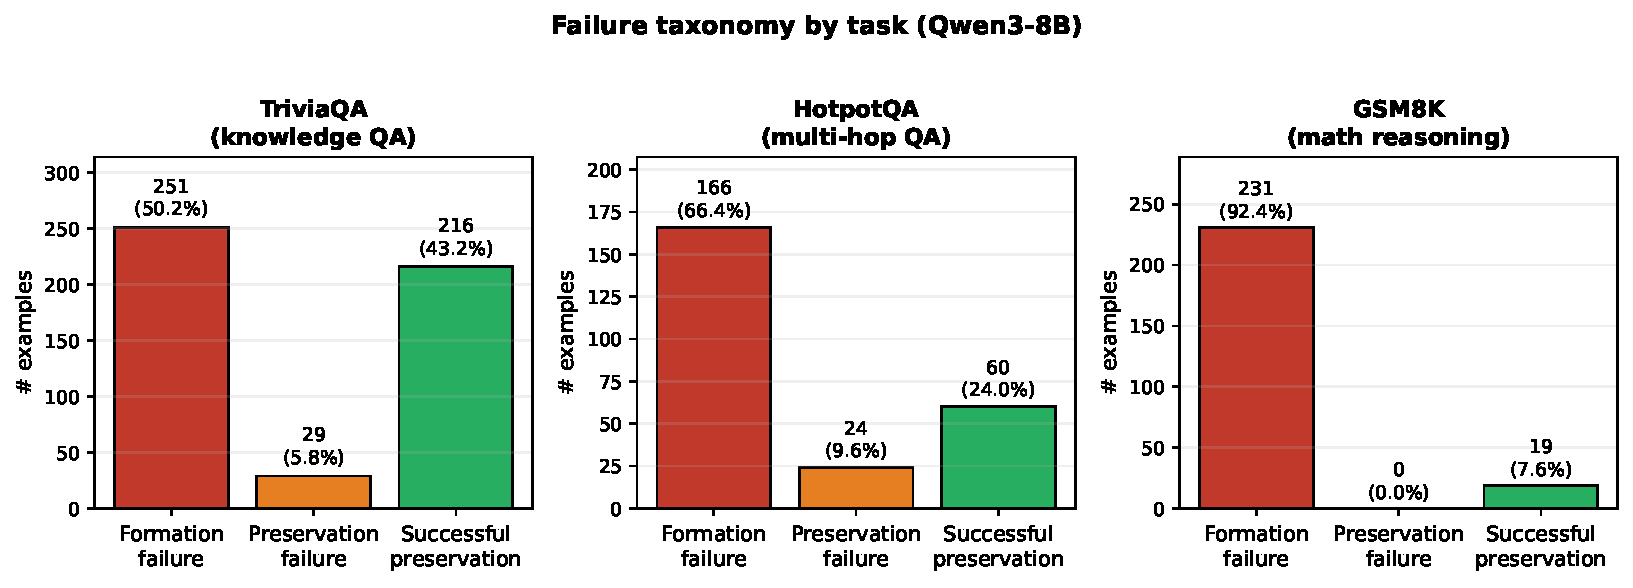
\includegraphics[width=0.85\textwidth]{figures/fig4_taxonomy.pdf}
\caption{Operational error taxonomy across tasks for Qwen3-8B under the strict criterion (Eq.~\ref{eq:tax}).}
\label{fig:taxonomy}
\end{figure}

\end{document}
